%!TEX root = ../main.tex

\chapter{Kravspecifikation}

\begin{table}[H]
\centering
{\rowcolors{2}{white!80!black!30}{white!70!black!60} %farver på hver anden række -starter på 3
\setlength{\arrayrulewidth}{0.2mm}					 %tykkelse på linier 
\setlength{\tabcolsep}{10pt}						 %indryk i celle 
\renewcommand{\arraystretch}{1.5}					 %højden på tabelrum
\center
\begin{tabular}{|p{4cm}|p{4cm}|p{4cm}|}		 %længden på alle rum
\hline

\multicolumn{3}{|>{\columncolor{white!20!black!90}}m{13.44cm}|}{\textcolor{white}{\large{\textbf{Revision}}}} \\\hline
\rowcolor{white!70!black!60}
\textcolor{black}{\large{\textbf{Ændret af}}}&
\textcolor{black}{\large{\textbf{Version}}}&	
\textcolor{black}{\large{\textbf{Dato}}}\\
\hline
Alle	& 1	 	& 23-02-2015  \\
		& 		&   \\
		& 		&   \\
		& 	 	&   \\
\hline
\end{tabular}
}
\caption{Revision for kravspec}
\label{table:RevKrav}
\end{table}



%Aktører
\section{Aktører}
%!TEX root = ../../main.tex

I dette afsnit beskrives aktører og deres rolle i systemet. I figur \ref{photo:Aktor} ses aktørdiagram, som beskriver alle aktører og deres forhold til systemet

\begin{figure}[H]
	\centering
	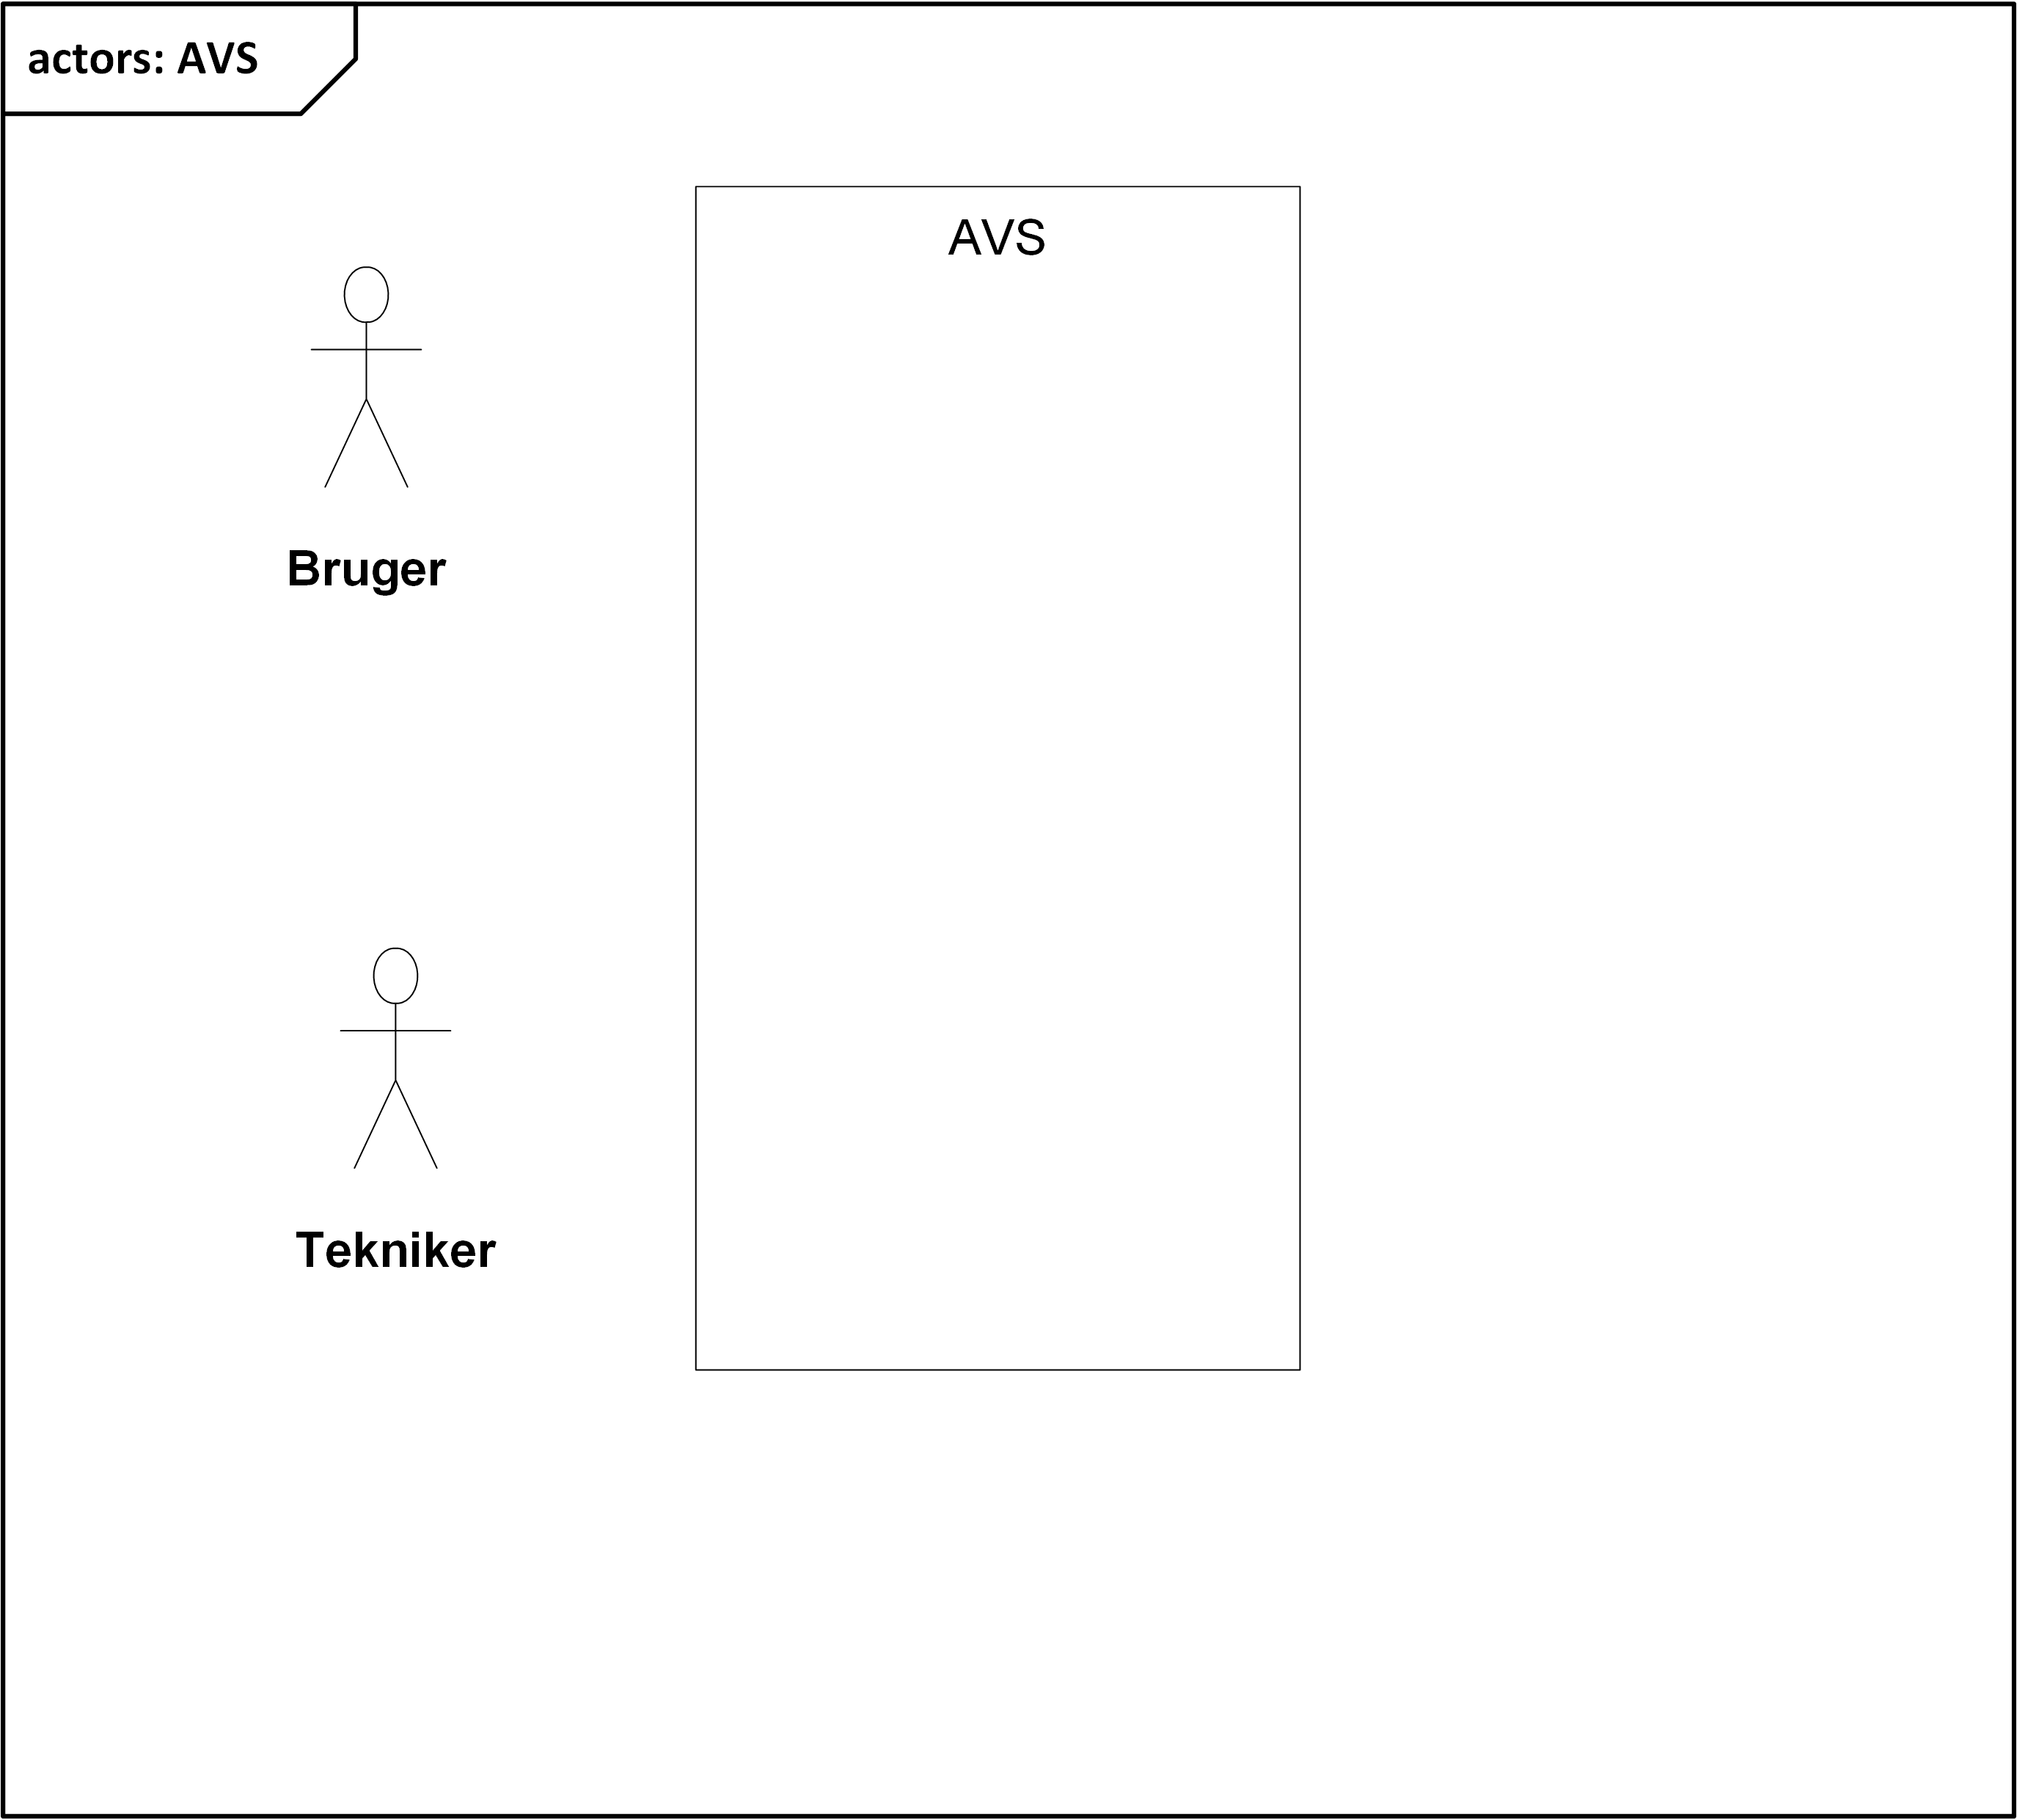
\includegraphics[scale=1]{Kravspecifikation/Actor/Photo/AVS_Actors}
	\caption{AVS Aktører}
	\label{photo:Aktor}
\end{figure}

\subsection{Bruger}
\begin{usecase}
\addtitle{Aktørnavn}{Bruger} 
\addfield{type:}{Primær}
\addfield{Beskrivelse:}{Brugeren er ham, som til dagligt tilgår systemet. Han ved hvor meget gødning og fugtighed planterne skal have, og angiver disse værdier i brugergrænsefladen. Det er brugeren som løbende ændrer værdierne, så systemet hele tiden er opdateret med værdier der passer til planternes vækststadier.}
\end{usecase}

\subsection{Tekniker}
\begin{usecase}
\addtitle{Aktørnavn}{Tekniker} 
\addfield{type:}{Primær}
\addfield{Beskrivelse:}{Teknikeren er en specielt uddannet person. Han har den nødvendige viden om systemet til at kunne installere systemet fra opstart, opsætte nye vandkar mv. En Bruger kan også være tekniker.}
\end{usecase}


\subsection{Planter}
\begin{usecase}
\addtitle{Aktørnavn}{Planter} 
\addfield{type:}{Sekundær}
\addfield{Beskrivelse:}{En plante, som systemet skal kunne vande. Planter består desuden også af et gromedie (jord, lega, mv.), som er det, der reelt bliver vandet.}
\end{usecase}



%Use Cases
\newpage
\section{Use Cases}
%	Indledning
I dette afsnit ses de forskellige use Cases. På billede \ref{photo:UseCD} ses et Use case diagram, som viser en simpel repræsentation af Bruger og Teknikers interaktion med systemet og en afbildning af de forskellig Use Cases. 
\newline
\begin{figure}[H]
	\centering
	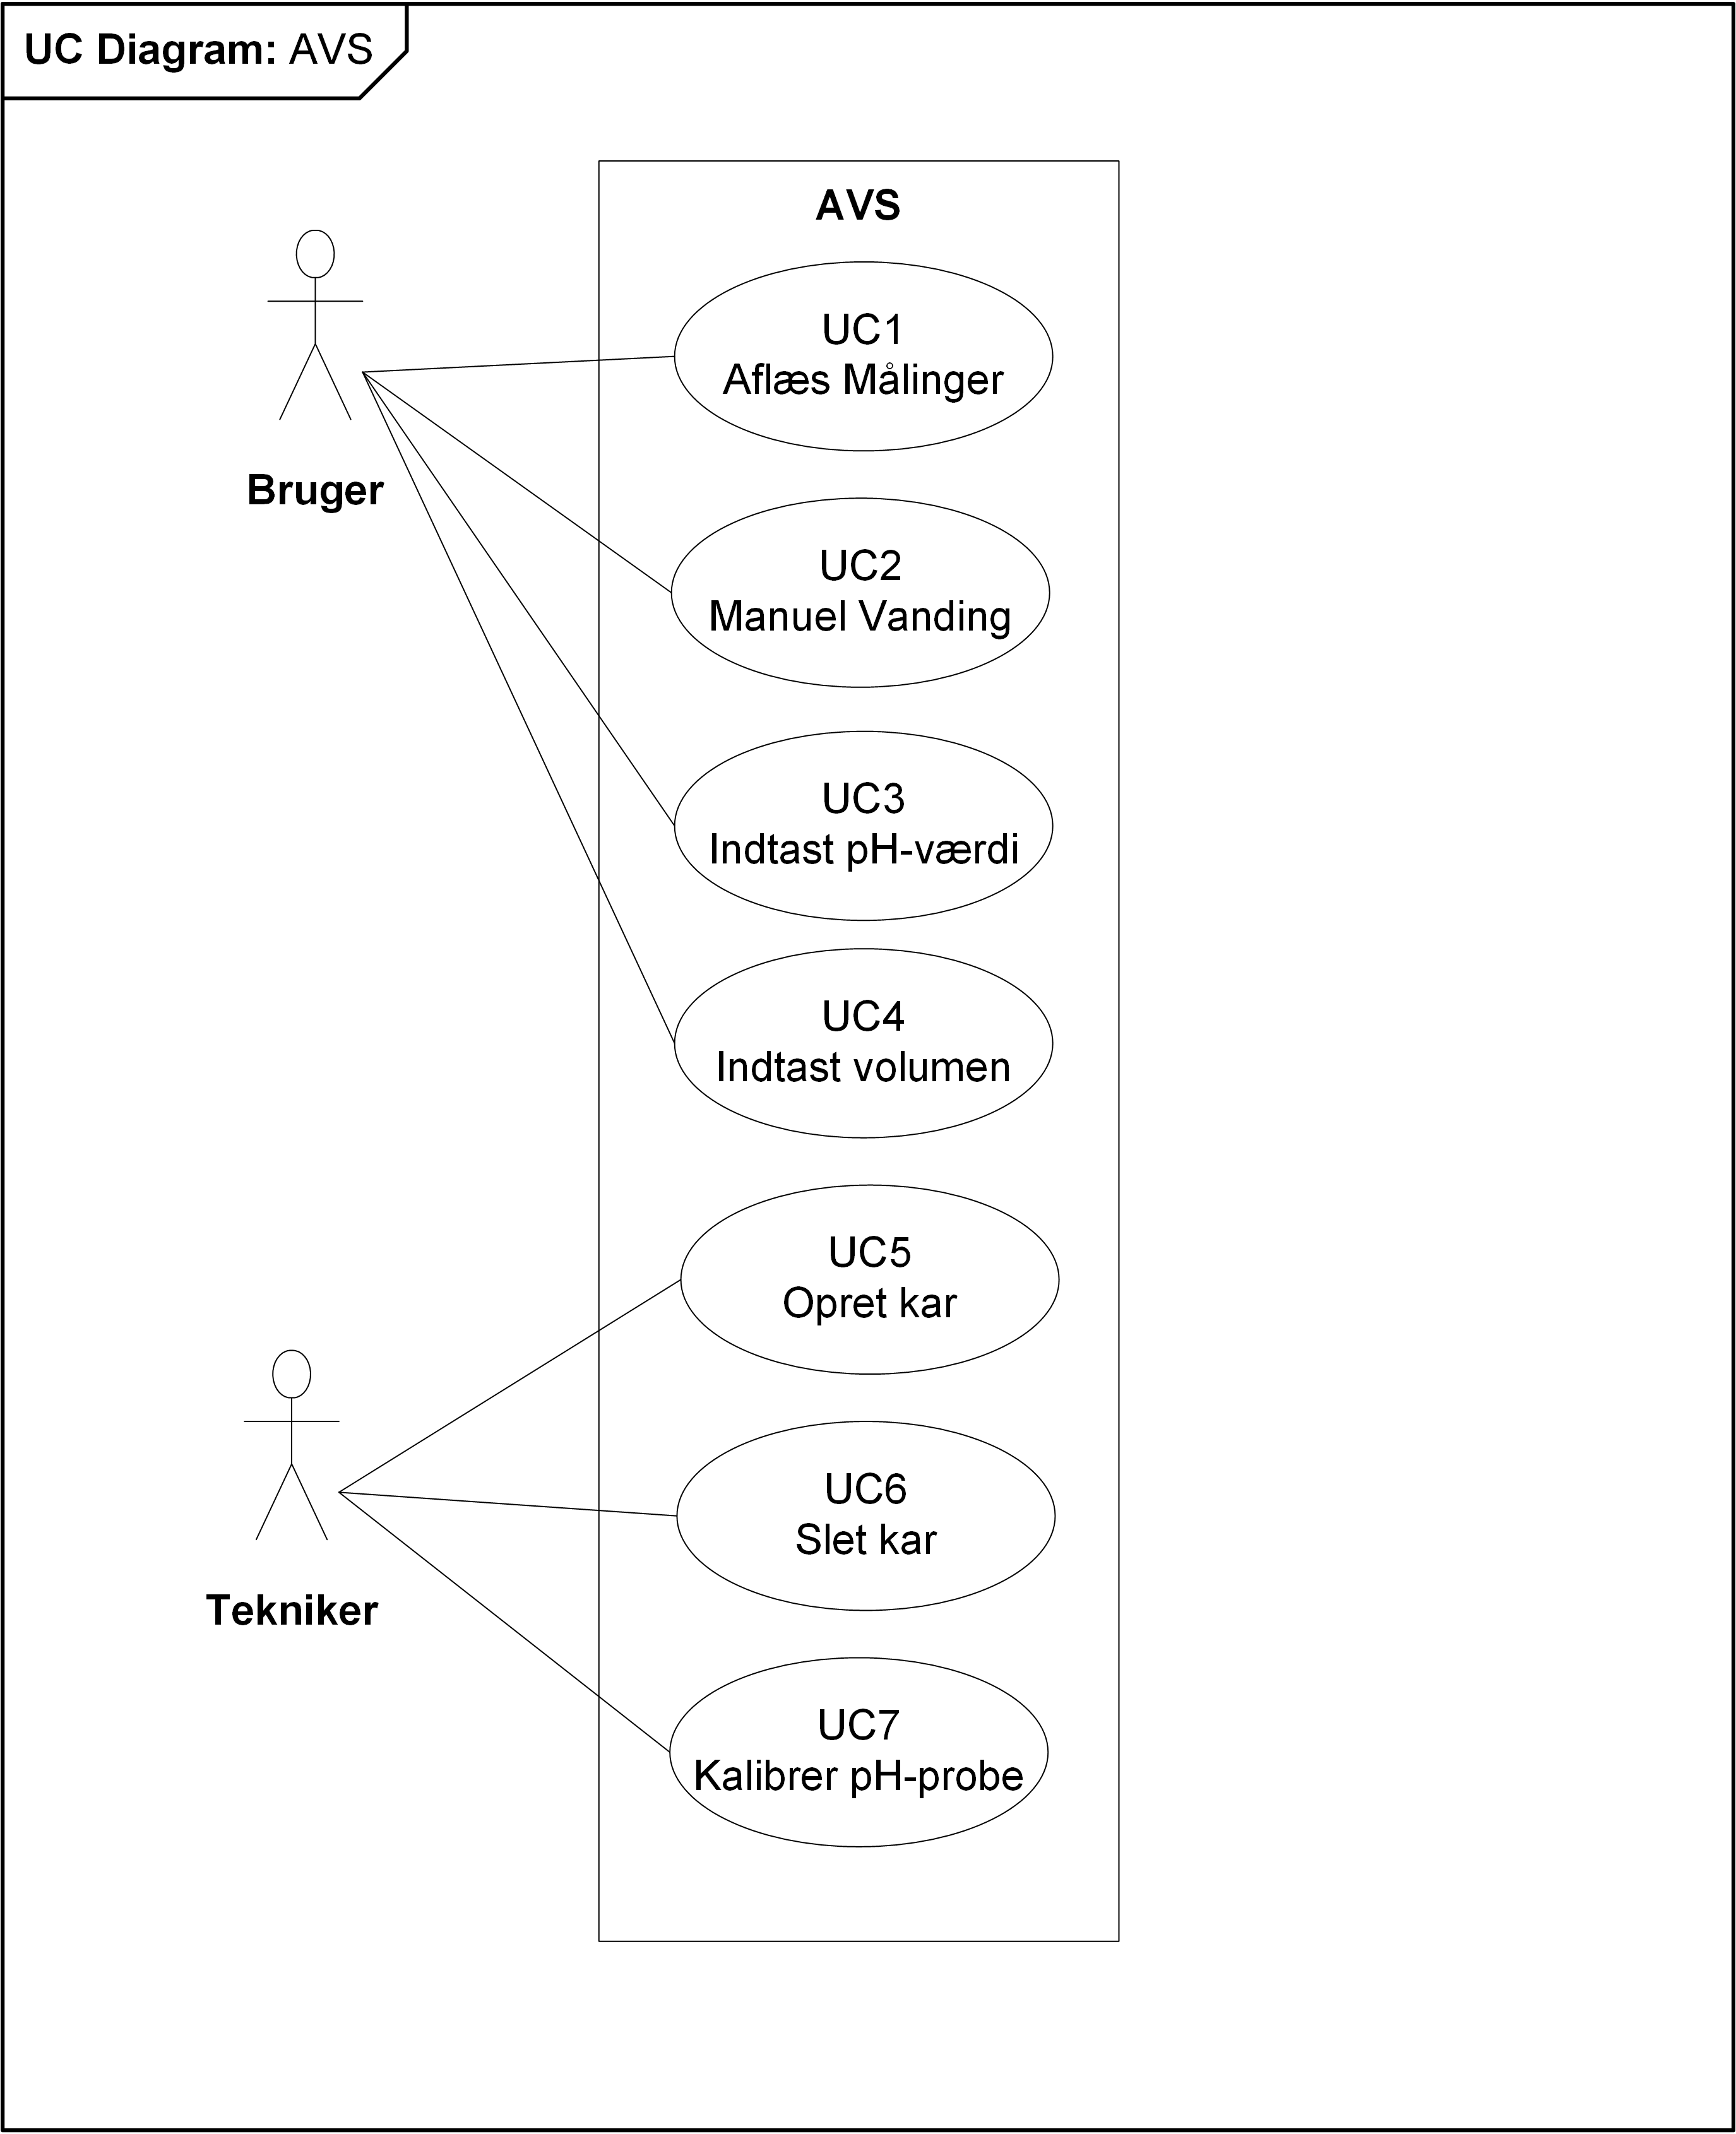
\includegraphics[scale=0.6]{Kravspecifikation/UseCases/Photo/AVS_UseCases}
	\caption{AVS Use case diagram}
	\label{photo:UseCD}
\end{figure}

\newpage
%	#1 Aflæs målinger
\subsection{Use case 1}
Når bruger ønsker at aflæse målingerne, skal data aflæses via \glslink{gui}{gui'en}. Denne use case kan kun gennemføres af en person. 



\begin{usecase}

\addtitle{Use Case 1}{Aflæs målinger} 

\addfield{Mål:}{Bruger aflæser ønskede målinger}

\addfield{Initieret af:}{Bruger}

\addfield{Aktør:}{Bruger}

\addfield{Samtidige forekomster:}{1 (inklusiv denne)}

%Preconditions: What must be true on start and worth telling the reader?
\addfield{Prækondition:}{Et fungerende system}

%Postconditions: What must be true on successful completion and worth telling the reader
\addfield{Postkondition:}{Målinger er aflæst af bruger}

%Main Success Scenario: A typical, unconditional happy path scenario of success.
\addscenario{Hovedscenario:}{
	\item Bruger trykker på "Kar X" i \gls{gui}
	\item Systemet viser et skærmbillede med oversigt over 	kar data.
	\item Bruger aflæser de ønskede målinger.
}

%Extensions: Alternate scenarios of success or failure.
%\addscenario{Extensions:}{
%	\item[2.a] Invalid login data:
%		\begin{enumerate}
%		\item[1.] System shows failure message
%		\item[2.] User returns to step 1
%		\end{enumerate}
%	\item[5.a] Invalid subsriber data:
%		\begin{enumerate}
%		\item[1.] System shows failure message
%		\item[2.] User returns to step 2 and corrects the errors
%		\end{enumerate}
%}


\end{usecase}

%	#2 Manuel vanding
\newpage
\subsection{Use case 2}
En bruger kan indtaste de ønskede data der er til de forskellige set-punkter. Denne use case kan kun styres af en bruger da der kun er en \gls{gui}. For at dette kan gennemløbes skal  systemet være operativt. Efter usecasen er gennemløbet forventes data at være indtastet og gemt i systemmet.   
\begin{usecase}

\addtitle{Use Case 2}{Indtast data} 

\addfield{Mål:}{Indtastet data for diverse setpunkter}

\additemizedfield{Initieret af:}{
	\item Bruger
	\item Tekniker
}

\additemizedfield{Aktør:}{
	\item Primær: Bruger
	\item sekundær: Tekniker
}

\addfield{Samtidige forekomster:}{1}

%Preconditions: What must be true on start and worth telling the reader?
\addfield{Prækondition:}{Systemet er operativt}

%Postconditions: What must be true on successful completion and worth telling the reader
\addfield{Postkondition:}{Data er indtastet}

%Main Success Scenario: A typical, unconditional happy path scenario of success.
\addscenario{Hovedscenarie:}{
	\item bruger tilgår systemet via \glslink{gui}{gui'en}
	\item Bruger indtaster ønskede data
	\item bruger gemmer værdier 	
}

\end{usecase}

%	#3 Indtast pH
\newpage
\subsection{Use case 3}
I denne use case ønsker brugeren at ændre på pH-værdien i karret. 
\begin{usecase}

\addtitle{Use Case }{Indtast pH-værdi} 

\additemizedfield{Mål:}{
\item At ændre pH-værdien på blandingen i karret 
}

\addfield{Initieret af:}{
	Bruger   
}

\additemizedfield{Aktører:}{\item Primær: Bruger}

\addfield{Samtidige forekomster:}{1}

%Preconditions: What must be true on start and worth telling the reader?
\addfield{Prækondition:}{Et kar er oprettet og systemet er funktionelt}

%Postconditions: What must be true on successful completion and worth telling the reader
\addfield{Postkondition:}{Systemet er opdateret med pH-værdi }

%Main Success Scenario: A typical, unconditional happy path scenario of success.
\addscenario{Hovedscenarie:}{
	\item Bruger trykker på "Kar X" i GUI
	\item Systemet viser et skærmbillede hvor det er muligt at indtaste en pH-værdi 	
	\item Bruger trykker på "pH-Værdi"
	\item Systemet viser en cursor i skrivefeltet tilhørende
	      pH-værdien
	\item Bruger indtaster en pH-værdi
	\item Bruger trykker på "Gem" 
	\item Systemet gemmer pH-værdien
}

%Extensions: Alternate scenarios of success or failure.
%\addscenario{Udvidelser:}{
%	\item[Ex.1] Teknikeren ønsker kun at aflæse værdier:
%		\begin{enumerate}
%		\item[1.] Teknikeren trykker på "OK"
%		\end{enumerate}
%}


\end{usecase}

%	#4 Indtast volumen
\newpage
\subsection{Usecase 4}
Karstyringen bliver anvendt til at styre vandkaret for at sikre at PH-værdien er vedligeholdt. Use casen kan kun køres af én af gangen, da der kun er et interface. For at use casen kan gennemløbes skal sensorer tilkoblet til systemet være funktionelle. Efter use casen er gennemløbet, er der indtastet en PH-værdi og en volumen på karet. Use casen har et main scenarie som er et happy path scenarie, samt en extension hvor teknikeren kun ønsker at aflæse værdier.
\begin{usecase}

\addtitle{Use Case 4}{Karstyring} 

\additemizedfield{Mål:}{
\item Styre vandkaret så en brugerdefineret PH-værdi holdes stabil i vandet
\item Sikre at der konstant er et flow i vandet
}

\addfield{Initieret af:}{
	Tekniker  
}

\addfield{Aktører:}{Primær: Tekniker}

\addfield{Samtidige forekomster:}{1}

%Preconditions: What must be true on start and worth telling the reader?
\addfield{Prækondition:}{Sensorer er tilkoblet og systemet er funktionelt}

%Postconditions: What must be true on successful completion and worth telling the reader
\addfield{Postkondition:}{Der er indtastet PH-værdi og volumen på karet }

%Main Success Scenario: A typical, unconditional happy path scenario of success.
\addscenario{Hovedscenarie:}{
	\item Teknikeren trykker på "Karstyring" på 				  					  interfacet 
	\begin{itemize}
	\item Ex.1 (Teknikeren ønsker kun at aflæse 				    					værdier)
	\end{itemize}	 	
	\item Teknikeren trykker på "PH-Værdi"
	\item Teknikeren indtaster en ønsket værdi
	\item Teknikeren trykker på "OK"
	\item Teknikeren trykker på "Volumen"
	\item Teknikeren indtaster en ønsket værdi
	\item Teknikeren trykker på "OK"
	\item Teknikeren trykker på "OK"
	\item Systemet opdaterer automatisk karets PH-værdi 
	\item Systemet starter for flow i vandet
}

%Extensions: Alternate scenarios of success or failure.
\addscenario{Udvidelser:}{
	\item[Ex.1] Teknikeren ønsker kun at aflæse værdier:
		\begin{enumerate}
		\item[1.] Teknikeren trykker på "OK"
		\end{enumerate}
}


\end{usecase}

%	#5 Opsæt kar
\newpage
\subsection{Use case 5}
I denne use case opretter Tekniker et nyt kar. 
\begin{usecase}

\addtitle{Use Case 5}{Opret kar} 

\additemizedfield{Mål:}{
\item At oprette et nyt kar i systemet
}

\addfield{Initieret af:}{
	Tekniker   
}

\additemizedfield{Aktører:}{\item Primær: Tekniker}

\addfield{Samtidige forekomster:}{1}

%Preconditions: What must be true on start and worth telling the reader?
\addfield{Prækondition:}{Ledig adresse på bussen i domæne 1}

%Postconditions: What must be true on successful completion and worth telling the reader
\addfield{Postkondition:}{Der er oprettet et kar}

%Main Success Scenario: A typical, unconditional happy path scenario of success.
\addscenario{Hovedscenarie:}{
	\item Tekniker trykker på "service" knap i \gls{gui}
	\item Systemet viser service menuen 
	\item Tekniker trykker på "Opret kar" i service menu
	\item Systemet viser en menu hvor det er muligt at
	      indtaste navn og adresse i et nyt kar 
	\item Tekniker indtaster navn i navnefeltet
	\item Tekniker indtaster adresse i adressefeltet
	\item Tekniker trykker "Opret kar"
	\item Systemet opretter det nye kar og sender Teknikeren til forsiden
	\item Det nye kar forekommer nu i hoved menuen
}

%Extensions: Alternate scenarios of success or failure.
%\addscenario{Udvidelser:}{
%	\item[Ex.1] Teknikeren ønsker kun at aflæse værdier:
%		\begin{enumerate}
%		\item[1.] Teknikeren trykker på "OK"
%		\end{enumerate}
%}


\end{usecase}

%	#6 Slet kar
\newpage
\subsection{Use case 6}
I denne use case sletter Tekniker et kar.
\begin{usecase}

\addtitle{Use Case 6}{Slet kar} 

\additemizedfield{Mål:}{
\item At slette et kar i systemet
}

\addfield{Initieret af:}{
	Tekniker   
}

\additemizedfield{Aktører:}{\item Primær: Tekniker}

\addfield{Samtidige forekomster:}{1}

%Preconditions: What must be true on start and worth telling the reader?
\addfield{Prækondition:}{Der er oprettet et kar i systemet}

%Postconditions: What must be true on successful completion and worth telling the reader
\addfield{Postkondition:}{Der er slettet et kar }

%Main Success Scenario: A typical, unconditional happy path scenario of success.
\addscenario{Hovedscenarie:}{
	\item Tekniker trykker på "Service" i GUI 
	\item Systemet viser service-menu
	\item Tekniker trykker på "Slet kar" knap
	\item Systemet viser en liste over oprettede kar
	\item Tekniker trykker på slet ud for det kar han ønsker at slette
	\item Systemet spørger om Teknikeren er sikker i en dialog
	\item Tekniker trykker "Ok"
	\item Systemet sletter karet
	\item Systemet returnerer Tekniker til listen over oprettede kar, og skriver at karret er slettet.
}

%Extensions: Alternate scenarios of success or failure.
%\addscenario{Udvidelser:}{
%	\item[Ex.1] Teknikeren ønsker kun at aflæse værdier:
%		\begin{enumerate}
%		\item[1.] Teknikeren trykker på "OK"
%		\end{enumerate}
%}


\end{usecase}

%	#7 Kalibrer pH-probe
\newpage
\subsection{Use case 7}
I denne use case kalibreres pH-proben, som er tilsluttet et kar. Dette skal gøres en gang hver måned samt ved oprettelse af et kar. Systemet viser selv en advarsel på forsiden med, at proben skal kalibreres, og viser hvilket kar den hører til.
\begin{usecase}

\addtitle{Use Case 7}{Kalibrer pH-probe} 

\additemizedfield{Mål:}{
\item At kalibrere en pH-probe
}

\addfield{Initieret af:}{
	Tekniker   
}

\additemizedfield{Aktører:}{\item Primær: Tekniker}

\addfield{Samtidige forekomster:}{1}

%Preconditions: What must be true on start and worth telling the reader?
\addfield{Prækondition:}{Systemet fremviser en advarsel med, at en pH-probe skal kalibreres. En rød LED lyser på styringen tilhørende pH-proben. Teknikeren er i besiddelse af buffer-væske med en pH-værdi på henholdsvis 4 og 7}

%Postconditions: What must be true on successful completion and worth telling the reader
\addfield{Postkondition:}{pH-proben er kalibreret og en grøn LED lyser på styringen tilhørende pH-proben }

%Main Success Scenario: A typical, unconditional happy path scenario of success.
\addscenario{Hovedscenarie:}{
	\item Tekniker holder trykknappen "Kalibrer" nede i 5 sekunder eller mere på styringen tilhørende pH-proben
	\item Rød LED på styringen til pH-proben blinker i et interval på 250ms 		
	\item Tekniker tager probe ud af karet og sætter den i buffer-væske med en pH-værdi på 7
	\item Tekniker venter i 5-10 minutter 
	\item Tekniker trykker på knappen "pH7" på styringen til 
		  pH-proben
	\item Styringen til pH-proben indlæser værdien fra proben
	\item Tekniker sætter proben i buffer-væske med en pH-værdi på 4
	\item Tekniker venter i 5-10 minutter 
	\item Tekniker trykker på knappen "pH4" på styringen til 
		  pH-proben
	\item Styringen til pH-proben indlæser værdien fra proben  
	\item Styringen til pH-proben giver besked til systemet om at proben er kalibreret  
	\item Styringen til pH-proben slukker for rød LED og tænder grøn LED 
	\item Systemet fjerner advarslen om at proben skal kalibrers 			
}

%Extensions: Alternate scenarios of success or failure.
%\addscenario{Udvidelser:}{
%	\item[Ex.1] Teknikeren ønsker kun at aflæse værdier:
%		\begin{enumerate}
%		\item[1.] Teknikeren trykker på "OK"
%		\end{enumerate}
%}


\end{usecase}

%	#Ikke fully dressed Use cases
\newpage
\section{Ikke fully dressed use cases}

\subsubsection*{Use Case 11 - Doser pH-væske}
I denne use case har Brugeren mulighed for at dosere pH-væske via en doseringspumpe indtil den ønskede pH-værdi er vist. 

\subsubsection*{Use Case 12 - Automatisk vanding}
I denne use case sker vandingen automatisk, baseret på den målte jordfugtighed. Hvis den målte jordfugtighed er for lav i forhold til den indtastede jordfugtighed, bliver der vandet ude ved sensor øerne, indtil den målte værdi ca. passer med den indtastede værdi.

\subsubsection*{Use Case 13 - Alarm}
Ved brugerdefineret grænseværdier (jordfugtighed, pH-værdi og volumen), afgiver systemet en alarm, f.eks. via. e-mail. 

\subsubsection*{Use Case 14 - Ugeplan}
I denne use case får Bruger mulighed for at indtaste en ugeplan for styring af dosering af pH-væske og vand til gromediet i løbet af ugen. 

\subsubsection*{Use Case 15 - Udprint log}
Bruger kan få udprintet en log over de hændelser der er forekommet i systemet, bla. sensordata og dosering af vand.


\newpage
\section{Ikke Funktionelle Krav}
Brugervenlighed:
\begin{itemize}
	\item Skal være intuitivt og let at opererer for udefrakommende:
	Der forudsættes en fungerende standard PC med Windows inkl. Explore/Chrome	/Firefox som browser

	\item Systemet skal kunne tilgås igennem en normal webbrowser:
		Her menes Explorer / Google Chrome / Firefox
	\item Systemet skal kunne tilgås over lokalt netværk samt over www
		Her forudsættes en fungerende internetopkobling og evt. lokalt netværk
\end{itemize}

Systembetingelser:
\begin{itemize}
	\item Systemet skal kunne fungere stabilt i temperaturintervallet (1 - 45$\degree$ C)
	\item Systemet skal kunne fungere stabilt under høj luftfugtighed (op til 50\%)
	\item Systemet skal være let at vedligeholde på daglig basis
		Systemets reservedele skal være lette at udskifte og skaffe.
\end{itemize}

Ydelse:
\begin{itemize}
	\item Systemet skal kunne fylde vandkarret på max. 2 min.
	\item Systemet skal kunne tømme vandkarret på max. 2 min.
	\item Systemet skal kunne dosere vand til gromediet med min 0,5 / max 2 liter/min.
	\item Systemet skal kunne dosere gødning til karret på max. 30 sek.
\end{itemize}

%Kravspecifikation